

\section{Cloud Computing}
A continuación se presentan las definiciones de algunos conceptos importantes relacionados a cloud computing.
\begin{itemize}
    \item Cloud : En cloud computing, la palabra cloud o nube es usado como metáfora para “internet”.
    \item Multitenencia : Es una sola instancia de software que corre en la infraestructura del proveedor y sirve a múltiples organizaciones de clientes. Este modelo se diferencia de las arquitecturas con múltiples instancias donde cada organización o cliente tiene su propia instancia instalada de la aplicación.
    \item Despliegue : Despliegue. Un despliegue de servicios es una instancia de un servicio alojado en el cloud, ya sea en un ambiente de pruebas, en un entorno de producción, o en ambos.
    \item Datacenter : Un datacenter es un edificio o sala de gran tamaño usada para mantener en él una gran cantidad de equipamiento electrónico. Suelen ser creados y mantenidos por grandes organizaciones con objeto de tener acceso a la información necesaria para sus operaciones.
    \item SOA : Es un paradigma de arquitectura para diseñar y desarrollar sistemas distribuidos. Las soluciones  SOA  han sido creadas para satisfacer los objetivos de negocio las cuales incluyen facilidad y flexibilidad de integración con otros sistemas, alineación directa a los procesos de negocio reduciendo costos de implementación, innovación de servicios a clientes y una adaptación ágil ante cambios incluyendo reacción temprana ante la competitividad.
    \item Escalabilidad : Un sistema informático es escalable si puede crecer para responder ante necesidades mas exigentes.
    \item Elasticidad: La elasticidad consiste en la potencia de escalar los
          recursos informáticos ampliándolos y reduciéndolos con una fricción mínima.
\end{itemize}


\section{Introducción}
Cloud computing, también llamado computación en la nube o servicios en la nube, es un paradigma que permite ofrecer servicios de computación a través de internet. Dichos servicios pueden ser por ejemplo redes, servidores, almacenamiento, aplicaciones.

Es un nuevo modelo de prestación de servicios de negocio y tecnología que permite al usuario acceder a un catálogo de servicios estandarizados y responder con ellos las necesidades de negocio, en forma flexible y adaptativa.
Permite aumentar el número de servicios basados en la red, esto genera beneficios tanto para los proveedores que pueden ofrecer de forma mas rápida y eficiente un mayor numero de servicios como para los usuarios que tienen la posibilidad de acceder a ellos. El acceso a los recursos es totalmente transparente e inmediato y mediante un modelo de pago por consumo, brindándole al usuario la sensación de poseer infinitos recursos.
\section{Modelos de Servicios}
Existen tres modelos de servicios que se pueden ver como capas sobre las cuales podían construirse y desplegarse aplicaciones distribuidas. Estas capas son infraestructura, plataforma y software.
En la figura (\ref{fig:Modelo_servicios})
podemos observar los distintos modelos y los respectivos controles de usuario y proveedor.

\begin{figure}[!ht]
    \centering
    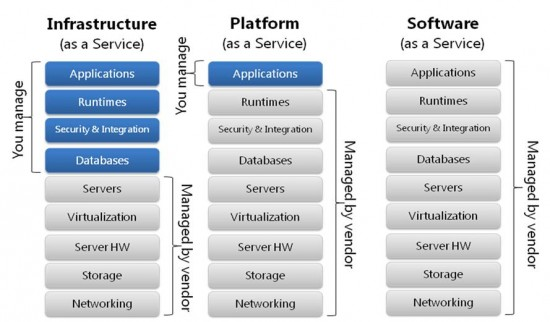
\includegraphics[width=\columnwidth, keepaspectratio]{_imagenes/Modelo_servicios.jpg}
    \caption{Mar Atlántico.} \label{fig:Modelo_servicios}
\end{figure}

\begin{description}
    \item[Cloud Software as a Service (SaaS).] El servicio provisto al usuario consiste en consumir una aplicación que es ejecutada en la nube, a demanda, vía multitenencia. Las aplicaciones que suministran este modelo de servicios son accedidas mediante un navegador web o de cualquier aplicación diseñada para tal efecto.
        El usuario no tiene control sobre la infraestructura de la nube, siendo transparente para el y eliminando la necesidad de instalar la aplicación en sus propias computadoras evitando costes de hardware y mantenimiento.

    \item[Cloud Platform as a Service (PaaS).] El servicio provisto al usuario consiste en utilizar la infraestructura de la nube para ejecutar aplicaciones desarrolladas por el usuario o adquiridas a terceros.
        Es el encapsulamiento de una abstracción del ambiente de desarrollo con sus modelos.
        El usuario no maneja ni controla la infraestructura de la nube, pero tiene control sobre la aplicación que es ejecutada y también sobre la configuración de entorno de ejecución de la aplicación.

    \item[Cloud Infraestructure as a Service (IaaS).] El servicio provisto al usuario consiste en la infraestructura de ejecución. El usuario es capaz de ejecutar código arbitrario, controla el sistema operativo y todas las aplicaciones de la nube.
        El hardware está virtualizado en la nube y se provee al usuario recursos como servidores, almacenamiento, redes, etc. Cada vez es mas adoptado este modelo, sobre todo por una gran cantidad de startups que lo utilizan por no poder permitirse tener datacenters propios. Provee mecanismos fáciles para que los desarrolladores interactúen con el IaaS generalmente creando máquinas virtuales. La interacción de las aplicaciones con IaaS suele ser a través de SOA con contratos de servicios, mediante WSDL o REST.
        Está dirigido a empresas que desean delegar la implantación de sus sistemas  en la infraestructura hardware de un proveedor externo, o servicios de almacenamiento externo, copias de seguridad de sus datos, cálculos complejos que requieran software de elevadas prestaciones, entre otros. El proveedor les permitirá gestionar dichos sistemas en un entorno virtualizado.

\end{description}

\section{Modelos despliegue}

Existen tren modelos de despliegue o tipos de cloud, el tipo de cloud a adoptar se debe definir en base a quien va a poder acceder a los servicios y a quien va a gestionar la infraestructura. Los tipos son privadas, públicas e híbridas y a continuación se explican cada una de ellas.

\begin{description}
    \item[Cloud privado] Una nube privada es aquella en la que solamente una organización, utilizando tecnologías como virtualización, tiene acceso a los recursos que se utilizan para implementar en la nube. Podría compararse con los datacenter que disponen algunas empresas, con infraestructura y máquinas propias dimensionadas en base a la demanda esperada. Mediante la virtualización se puede añadir a las características de los datacenters los beneficios del cloud como la agilidad de provisión o cierto nivel de elasticidad.
        La principal ventaja es que generan seguridad para los clientes, ya que no comparten recursos con otros usuarios. La capacidad de elegir el proveedor permite a los clientes seleccionar los recursos tecnológicos que mejor se adapten a sus necesidades técnicas y económicas.
        La desventaja que presenta este modelo es que al ser infraestructuras dedicadas al autoconsumo, el "pago por uso" no es un beneficio directo, ya que los recursos no utilizados no se revenden a otras organizaciones.
        Así, las nubes privadas están especialmente orientadas a organizaciones con alta concentración de recursos y sistemas tecnológicos, tales como entidades bancarias, Administración Pública, entornos de investigación y desarrollo, consultorías y asesorías legales, tecnológicas o de negocio, etc.

    \item[Cloud público]
        Una nube pública (o Cloud multi-tenant) se caracteriza por ofrecer recursos  sobre infraestructuras compartidas entre múltiples clientes. A estos recursos el cliente accede a través de internet o mediante conexiones VPN. La infraestructura es proporcionada con todas las ventajas del modelo de consumo de Cloud (pago por uso, aprovisionamiento ágil, elasticidad, etc.) beneficiándose además de las economías que se aplican al amortizar la infraestructura global con múltiples clientes.
        La ventaja más clara es que se adquiere poder de procesamiento y almacenamiento sin requerir inversión inicial, ya que se paga por lo que se usa. La desventaja se encuentra por el acceso al servicio a través de terceras empresas. También puede ser difícil integrar estos servicios con otros sistemas propietarios.

    \item[Cloud híbrido]
        Es un despliegue que combina recursos de cloud públicos y privados. Surge de la necesidad de los clientes de a pesar de tener su propia infraestructura buscar aprovechar las ventajas de los servicios de proveedores externos.
        Esto permite a una empresa mantener el control sobre las aplicaciones críticas para su negocio y aprovechar al mismo tiempo las posibilidades ofrecidas por los servicios ofertados por la nube en aquellas áreas donde resulte más adecuado. Aportan agilidad y reducción de costes sacrificando algo de control pero son una solución compleja, ya que requiere coordinación entre una infraestructura propia con otra gestionada por otro entorno.

\end{description}

\section{Ventajas y desventajas del cloud}
\subsection {Ventajas del uso de cloud}
Las ventajas que presenta el uso de la nube son varias y están asociadas a las necesidades y capacidades del cliente. Una de las ventajas más notables es como se mencionó es el modelo "paga por lo que uses", mediante la utilización de este modelo se presenta una ventaja al cliente, ya que paga solamente los recursos que utiliza y el proveedor tiene la ventaja que puede brindar los recursos que no son utilizados a otros clientes. A esto también le podemos sumar el ahorro por los gastos de infraestructura y mantenimiento. \\
El uso del cloud permite a Empresas no tan desarrolladas poder competir en cuanto a uso de tecnologías con otras más desarrolladas, teniendo acceso a últimas tecnologías y equipos costosos que sin el uso de la nube no podrían tenerlos.

Los datos pueden ser accedidos desde cualquier parte del mundo y con un acceso tolerante a fallos, lo que es beneficioso para los clientes que desean poder acceder a sus datos en todo momento.
Otra ventaja importante es la escalabilidad, en el uso de cloud la escalabilidad es transparente al cliente y en caso de necesitar más recurso de procesamiento o almacenamiento el proveedor se lo dará casi en tiempo real.
Se adecua al tiempo de mercado, por eso es utilizado por una gran cantidad de pequeñas empresas que recién comienzan, ya que sin la necesidad de una gran inversión pueden comenzar a trabajar tempranamente.

\subsection {Desventajas del uso de cloud}
Si bien como mencionamos anteriormente son muchas las ventajas que presenta el uso del cloud, también existen posibles desventajas.
La más clara tal vez es la privacidad, para muchos clientes es difícil confiar su información sensible a terceros dejando de tener control sobre ellos.
Otra desventaja es la disponibilidad, si bien se encuentra en la sección ventajas, también es una desventaja, ya que la disponibilidad tiene una fuerte dependencia con internet, sin internet no hay nube. También porque es el proveedor el encargado de proveer disponibilidad, pero si su tolerancia a fallos falla el cliente no puede hacer nada hasta que el proveedor lo solucione, existe una dependencia entre la disponibilidad y el proveedor.
Otra desventaja es que si un cliente desea cambiar de proveedor por cualquier motivo, no se puede garantizar el perfecto funcionamiento de su sistema. Esto se da porque no existe un estándar entre implementaciones de la nube por lo que la compatibilidad no está garantizada.

\section{Arquitecturas en la nube}
Para poder sacar provecho a una infraestructura escalable es de vital importancia que la arquitectura sea escalable. La nube está diseñada para proporcionar escalabilidad desde un punto de vista conceptual, sin embargo no se podrá aprovechar toda la escalabilidad de la infraestructura si la arquitectura del sistema no es escalable. Ambas deben trabajar mano a mano, debiendo identificarse los cuellos de botella y adecuando la misma con el objetivo de aprovechar la infraestructura escalable. A continuación se listan algunas de las características que se deben tener en cuenta a la hora de diseñar una arquitectura escalable:

\begin{itemize}
\item El aumento de recursos deriva en un aumento proporcional del rendimiento.
\item Un servicio escalable es capaz de gestionar la heterogeneidad.
\item Un servicio escalable es eficiente desde un punto de vista operativo.
\item Un servicio escalable es sólido.
\item Un servicio escalable debe ser más rentable cuando crece
\end {itemize}

La elasticidad dentro de una arquitectura es una noción pura del paradigma cloud, ya que la idea de poder contar con nuevos recursos en cuestión de minutos era imposible. La informática de nube optimiza el proceso de adquisición de los recursos necesarios. Ya no hay que realizar pedidos con antelación ni conservar hardware no utilizado. Ahora, los arquitectos de
la nube pueden solicitar los recursos que necesitan minutos antes de necesitarlos o automatizar el proceso de obtención, aprovechando la enorme escalabilidad y el rápido tiempo de respuesta.
La tolerancia a fallos y confiabilidad también son características deseables en arquitecturas cloud. La tolerancia a fallos es la capacidad del sistema de recuperarse y volver a un estado estable ante eventuales errores. La confiabilidad es disponer del correcto funcionamiento de todos los componentes al trabajar en conjunto.



\section{Ejemplo Cloud - Microsoft Azure}

Azure es la plataforma en la nube de Microsoft. Es una colección creciente de servicios integrados (proceso, almacenamiento, datos, red y aplicaciones).
Provee servicios siguiendo los modelos SaaS, PaaS e IaaS y la eficaz combinación de los servicios administrados y sin administrar permiten crear, implementar y administrar aplicaciones para obtener una buena productividad. Permite la posibilidad de tener un despliegue híbrido. Es abierto y flexible admitiendo cualquier sistema operativo, lenguaje, herramienta y marco, ya sea Windows, Linux, SQL Server, Oracle, C sharp o Java. Además, pone a su alcance lo mejor de los ecosistemas de Windows y Linux, por lo que puede se pueden crear excelentes aplicaciones y servicios que funcionan con cualquier dispositivo.
La plataforma Azure es más que servidores virtuales en varios centros de datos distribuidos estratégicamente. En la figura (\ref{fig:architectureazure}), se expone la arquitectura de la plataforma Azure y a continuación se detallan en cada uno de los mismos.

\begin{figure}[h!]
    \centering
    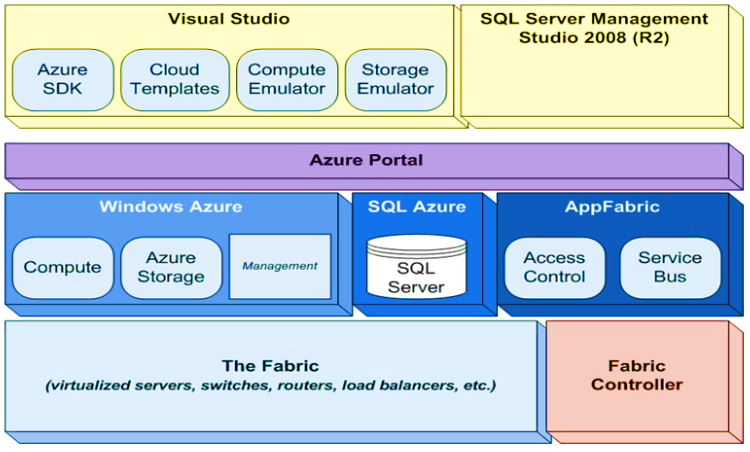
\includegraphics[width=\columnwidth, keepaspectratio]{architectureazure}
    \caption{Arquitectura de la plataforma Azure}   \label{fig:architectureazure}
\end{figure}



\begin{description}
    \item [The Fabric.] Se refiere principalmente a los componentes físicos que hacen posible la interoperabilidad entre sistemas, algunos de ellos como: servidores, switches, routers, etc. Fabric puede ser un sinónimo de centro de datos Microsoft.

    \item [Fabric Controller.] Esencialmente es software que opera bajo el modelo de controladores, utiliza drivers para cada componente de la fábrica además de administrar la implementación de servicios y almacenamiento de datos.

    \item [Windows Azure.] Se puede ver como el sistema operativo de la nube y se divide en tres servicios:
          \begin{itemize}
              \item Compute : Es el ambiente de ejecución donde aplicaciones y servicios ejecutan procesos computacionales, cualquier cloud service que se publique en Azure, se ejecutará aquí.
              \item  Storage : Es el ambiente para almacenar datos, se refiere a los tipos de almacenamientos en la nube (tablas, colas y blobs).
              \item Management : Infraestructura automatizada y administrada de los servicios en la nube.  El servicio de management es el fabric controller más otras funcionalidades.
          \end{itemize}

    \item [SQL Azure.] Es el sistema de gestión de base de datos relacional en la nube, es una versión modificada de SQL Server 2008.

    \item [AppFabric.] Es un componente clave que ofrece tres servicios:

          \begin{itemize}
              \item Access Control: Autenticación y permisos hacia las aplicaciones.
              \item  Service Bus: Mensajería segura y conectividad dentro y fuera de la nube.
              \item Caching Service: Cache para aplicaciones Azure.
          \end{itemize}

    \item [Portal Azure.] Portal web que permite la administración de todos los recursos que ofrece la plataforma Azure.

    \item [Herramientas.] Ambientes de desarrollo para la implementación de soluciones en la nube como Visual Studio o SQL Server Management Studio.

\end{description}

Los servicios son provistos mediante servicios REST mediante una REST API permitiendo acceder a los servicios a través de una plataforma web o consola. La configuración y control de los servicios se puede realizar a través del portal web Microsoft Azure Portal, con una interfaz sencilla y amigable, facilitando el uso a los usuarios y pudiendo accederla desde cualquier browser. De este modo el usuario no necesita instalar ningún componente para poder configurar y controlar los servicios. En cambio si se desea desarrollar aplicaciones para Azure si es necesario instalar ciertos componentes para la correcta depuración de la aplicación.


\subsection {Modelos de ejecución}
En Azure existen tres modelos de ejecución para proveer servicios al cliente. Ellos son Web Sites, Cloud Services y Virtual Machines. Cada modelo provee a su vez un conjunto de servicios y la elección de cual usar  por parte del cliente depende de las necesidades del mismo. A continuación detallamos cada uno de los mismos.

\begin{description}
\item [Virtual Machines.] Permite crear y usar máquinas virtuales en la nube y así provee IaaS.

\begin{figure}[h!]
    \centering
    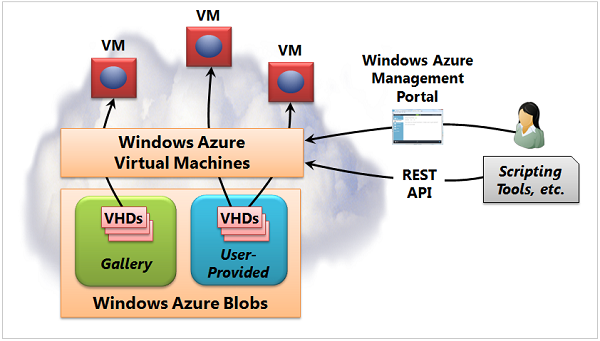
\includegraphics[width=\columnwidth, keepaspectratio]{_imagenes/azure_virtualmachines}
    \caption{Máquinas virtuales en Azure para proveer IaaS} \label{fig:azure_virtualmachines}
\end{figure}

El usuario puede crear y controlar máquinas virtuales desde el portal web o utilizando la REST API que mencionamos anteriormente. Al crear  una máquina virtual se debe elegir un disco duro virtual (VHD). Para esto existen dos opciones, una es que el usuario suba su propio VHD y la otra es usar uno nuevo que provee Microsoft en la galería de máquinas virtuales. Estos discos se guardarán en  Azure Blobs, se presentarán estos componentes más adelante. Los VHDs en la galería cuentan con imágenes de sistemas operativos Windows y Linux con productos ya instalados. Entre las configuraciones posibles se encuentran Windows Server, Linux servers, SQL server, BizTalk Server, SharePoint Server. También se debe seleccionar el tamaño que tendrá la máquina virtual, para esto se brindan configuraciones de memoria y cores los cuales debe seleccionar el usuario. Las configuraciones posibles son:

\begin{itemize}
\item Extra Small, con core compartido y  768MB de memoria.
\item Small, con 1 core y 1.75GB de memoria.
\item Medium, con 2 cores y 3.5GB de memoria.
\item Large, con 4 cores y 7GB de memoria.
\item Extra Large, con 8 cores y 14GB de memoria.
\item A6, con 4 cores y 28GB de memoria.
\item A7, con 8 cores y 56GB de memoria.

\end {itemize}
Por último se debe configurar sobre que datacenter correrá la máquina virtual creada siendo Estados Unidos, Asia o Europa las opciones.\\
Luego de creada la máquina virtual el pago se realiza por hora de trabajo.

\item [Web Sites.] Utiliza el modelo PaaS y permite desarrollar, deployar y escalar aplicaciones web. Se utiliza cuando el usuario no necesita tener control sobre la máquina virtual donde corre su aplicación, delegando dicho control a Azure.

\begin{figure}[h!]
    \centering
    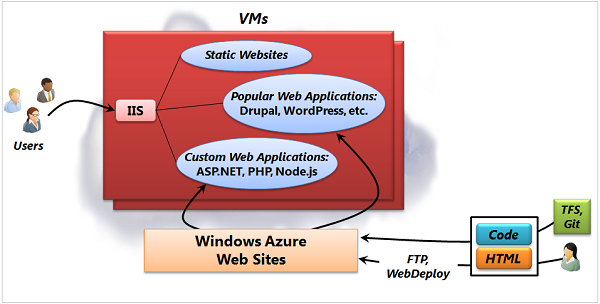
\includegraphics[width=\columnwidth, keepaspectratio]{_imagenes/azure_websites}
    \caption{WebSites en Azure para proveer PaaS} \label{fig:azure_websites}
\end{figure}

Web Sites de Azure permite tanto la creación de nuevos sitios, como la migración de sitios ya existentes. En ambos casos es posible configurar el escalado del sitio según los criterios definidos.
El usuario tiene la posibilidad de optar si desea utilizar una máquina virtual para el solo o una compartida y provee templates, frameworks y herramientas para el fácil y rápido desarrollo de aplicaciones web. La tecnología da soporte para la creación de aplicaciones usando ASP.NET, PHP, Node.js y Python.
Aplicaciones creadas en WebSites también pueden usar otras funcionalidades de Azure como Service Bus, SQL Database, y Blob Storage.\\
Para la publicación del sitio se puede realizar mediante FTP, FTPS o tecnología de Microsoft para deploy. También desde sistemas de source control como Git, GitHub, Bitbucket, Dropbox, Team Fundation Server.

Azure Websites no solo funciona con aplicaciones web, también se pueden realizar tareas de cómputos utilizando WebJobs.


\item [Cloud Services.] Cloud Services es otro ejemplo de PaaS. Al igual que WebSites está desarrollado para soportar aplicaciones escalables. Si bien los clientes no tienen control absoluto sobre las máquinas virtuales, tienen mas control que usando WebSites.



La tecnología provee dos opciones de virtualización, una basada en web roles que ejecutan un similar a Windows Server con IIS mientras que la otra opción es ejecutar web roles, también similar a Windows Server pero sin IIS. Por ejemplo una aplicación simple puede ejecutar solo en un web role pero si la aplicación es compleja además de ejecutar en web role se puede pasar trabajo a worker roles.

\begin{figure}[h!]
    \centering
    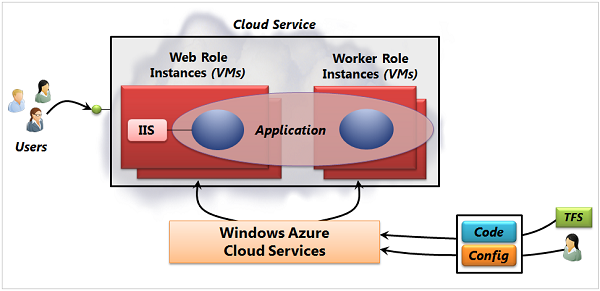
\includegraphics[width=\columnwidth, keepaspectratio]{_imagenes/azure_cloudservices}
    \caption{Cloud Services en Azure} \label{fig:azure_cloudservices}
\end{figure}

\end{description}


\red{faltan referencias}
La elección del modelo a utilizar es fuertemente dependiente de las características del problema a resolver. Si se desea por ejemplo una aplicación con poca configuración y acceso a base de datos, Web Sites es la opción que mejor se adapta a estas necesidades. Por otro lado, si se desea crear una arquitectura con mas de una capa que ejecute aplicaciones con gran nivel de computo y específicas condiciones de escalado, Cloud Services es la opción correcta. En cambio, si se desea instalar en el cloud una aplicación que requiere gran configuración del sistema operativo subyacente, la mejor opción en este caso sera utilizar Virtual Machines.

\subsection {Modelos de almacenamiento}
\red{faltan referencias}
El acceso a datos en Azure se realiza mediante servicios RESTful pudiendo realizar llamados desde consola o aplicación web. Desde el portal también se pueden crear las cuentas de almacenamiento de forma rápida y sencilla. La cantidad de cuentas de almacenamiento que puede crear el usuario está limitado por el tipo de cuenta de Azure que el usuario posee. Azure provee cuatro opciones para el manejo de almacenamiento, blobs, tables, queues y drives o unidades.

\begin{description}

    \item [Blobs.] Un Blob es un archivo de cualquier tipo. Existen dos tipos, Block y Page Blob. Block Blob es optimizado para el uso de streaming de datos mientras que Page Blob es optimizado para la realización de operaciones de lectura / escritura.Los blobs se alojan en Containers, pudiendo tener una cantidad ilimitada de Blobs respetando los tamaños máximos de almacenamiento permitido. El acceso a un Blob se realiza utilizando la URL con el formato
          http://[storageAccount].blob.core.windows.net/[container]/[blob]

          \red{faltan referencias}
    \item [Tables.] Permite almacenar gran cantidad de datos estructurados. Una tabla es definida dentro de una cuenta de almacenamiento pero no dentro de un Container y esta conformada por un conjunto de entidades. La diferencia entre las tablas de Azure y las de base de datos relacionales es que las tablas de Azure no posee esquema de entidades, por lo que entidades de una misma tabla pueden poseer distintas propiedades.

          \red{faltan referencias}
    \item [Queues.] Permite almacenar una gran cantidad de mensajes que pueden ser accedidos utilizando llamados HTTP o HTTPS autenticados. Pueden actuar como una forma de enrutar trabajo entre los diferentes roles dentro de una aplicación de una forma durable y escalable.

          \red{faltan referencias}
    \item [Drives.] Son espacios NTFS donde podemos utilizar las APIs tradicionales de lectura y escritura. La diferencia de utilizar un servicio de drive o utilizar el drive de la máquina virtual es que el servicio de drive está disponible para todos los roles y preparado para escalar.


\end{description}

\subsection {HDInsight}
\red{faltan referencias}
HDInsight es un servicio de Azure que provee y despliega clústers de Apache Hadoop \cite{hadoop} en el cloud, brindando un framework para analizar, manejar y reportar grandes volúmenes de datos, ofreciendo así una implementación del model MapReduce de Apache Hadoop para el análisis de big data. Los clusters Hadoop en HDInsight utilizan una versión de Hortonworks Data Platform(HDP) y un conjunto de componentes de Hadoop de dicha distribución. En la versión actual de HDInsight, la 3.1,   la versión 2.1.7 de HDP y 2.4.0 de Apache Hadoop. En HDInsight el sistema de archivos de Hadoop (HDSF) se almacena como Blobs en un Container asociado al cluster en la cuenta de almacenamiento.\\

\begin{figure}[h!]
    \centering
    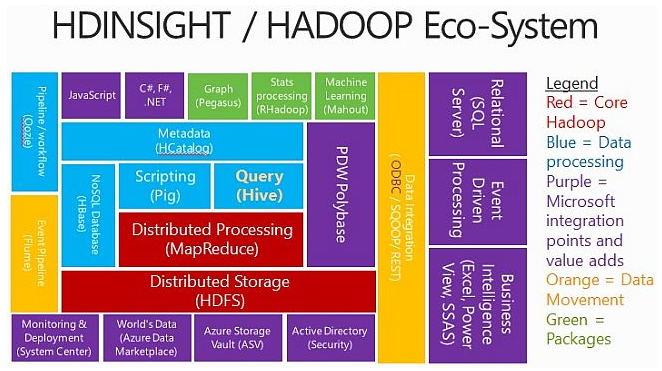
\includegraphics[width=\columnwidth, keepaspectratio]{HDInsight}
    \caption{Ecosistema HDInsight / Hadoop}
    \label{fig:HDInsight}
\end{figure}
